\documentclass[12pt]{article}
\usepackage{array}
\usepackage{amsmath}
\usepackage{mathtools}
\usepackage{gensymb}
\usepackage{graphicx}
\usepackage{float}

\allowdisplaybreaks

\begin{document}
    \title{The Maximum Range and Optimal Launch Angle of a Projectile Launcher at a Particular Height}
    \author{Ryan Coyne}
    \maketitle
    \section{Abstract}
        \paragraph{}The maximum range of a projectile launcher at a particular height and the launch angle 
        at which that range is reached, referred to as the optimal launch angle from here out, was measured using meter 
        sticks. The theoretical maximum range was (\(4.69 \pm 0.13\)) m and the theoretical optimal launch angle was 
        (\(38.04 \pm 0.18\))\(\degree\).
    \section{Introduction}
         \paragraph{}This experiment determined the maximum range and optimal launch angle of a spring loaded projectile launcher at a 
         particular height. The range, $R$, is the displacement of the projectile in the horizontal direction and is dependant 
         on the launch angle, $\theta$, launch height, $y_0$, and initial velocity, $v_0$.  The maximum range depends on the height that the projectile is 
         launched from because when launched from 
         a greater height the projectile spends more time in the air and therefore has more time to travel horizontally. The 
         optimal launch angle decreases as the launch height increases because the extra time in the air that is gained from a 
         greater launch angle will be less significant than the extra air time gained from being launched from higher above the ground 
         and therefore it will be more effective to add to the horizontal velocity at the cost of the vertical velocity. $R$ can be 
         Calculated
         \begin{center}
             \(R = \frac{v_0 \cos(\theta)}{g}\left(v_0 \sin(\theta) +\sqrt{(v_0 \sin(\theta))^2-2gy_{0}}\right)\)
         \end{center}
         Extremizing, $R$, gives us the maximum range, $R_{max}$, and the optimal launch angle, $\theta_{max}$. 
    \section{Procedure}
        \paragraph{}A spring loaded projectile launcher was clamped to a table. The launcher has the location of the center of the 
        ball that is being launched at the time it is no longer in contact with the launcher marked. This marking is also 
        the axis that the launcher rotates around to achieve different launch angels. The distance from the center of the 
        ball at the time of launch to the floor was measured. The launcher uses a string 
        with a small metal ball tied to the end in combination with markings on the side of the launcher to show the angle 
        that the launcher is tilted to relative to the ground. It also has three speed settings based on how far the 
        spring is retracted. A string tied to a plumbob was held to the launcher and the 
        distance from the center of the ball at launch to the string was measured and then that distance from the plumbob 
        toward the launcher was measured and marked with tape. The launcher was set to a launch angle of zero degrees and 
        a ball was inserted into the launcher at the maximum speed setting. The ball was then launched and a piece of 
        paper was taped to the ground in approximately the location that the ball landed. A piece of carbon paper was 
        placed over the taped paper and the ball was launched with the same process four more times, each time landing 
        on the carbon paper and making a mark on the paper beneath. Next meter sticks were placed end to end on the floor 
        to measure the distance between the tape used to mark the center of the ball at the time of launch to the marks 
        made by the ball landing on the carbon paper. 
        \paragraph{}The optimal launch angle and maximum range were determined from the ranges in the four trials at 
        the launch angle of zero degrees. Next three sets of four trials were conducted using the same method outlined 
        above but at the optimal launch angle, the optimal launch angle plus ten degrees, and the optimal launch angle 
        minus ten degrees. \\
        \begin{figure}[h]
            \caption{Figure 1. Experimental Setup}
            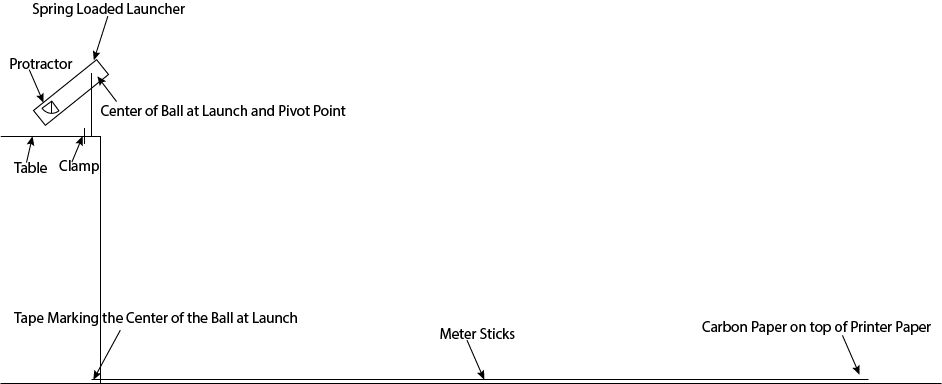
\includegraphics[width=\linewidth]{Setup.png}
        \end{figure}
    \section{Data}
        \begin{center}
            \begin{tabular}{>{\centering\arraybackslash}p{0.07\textwidth}|>{\centering\arraybackslash}p{0.1\textwidth}>{\centering\arraybackslash}p{0.1\textwidth}}
                \multicolumn{3}{c}{Table 1. Determining \(v_0\)}\\ 
                Trial & $y_0 \ (\text{m})$ & $R_0 \ (\text{m})$ \\
                \hline
                1 & 1.1631 & 2.864\\
                2 & 1.1629 & 2.906\\
                3 & 1.1625 & 2.963\\
                4 & 1.1628 & 2.965\\
                \hline
                \(\overline{x}\) & 1.16283 & 2.925\\
                \(\sigma\) & 0.00025 & 0.049
            \end{tabular}\\[12pt]
            \begin{tabular}{c|ccc}
                \multicolumn{4}{c}{Table 2. Testing Preditictions of Maximum Range}\\
                 Trial & $R(\theta_{Max}) \, (m)$ & $R(\theta_{Max} + 10 \degree)\, (m)$ & $R(\theta_{Max}-10 \degree)\, (m)$\\
                 \hline
                 1 & 4.801 & 4.505 & 4.515\\
                 2 & 4.783 & 4.500 & 4.505\\
                 3 & 4.750 & 4.490 & 4.485\\
                 4 & 4.742 & 4.440 & 4.475\\
                 \hline
                 \(\overline{x}\) & 4.769 & 4.484 & 4.495\\
                 \(\sigma\) & 0.028 & 0.030 & 0.018 
            \end{tabular}\\[12pt]
            \begin{tabular}{>{\centering\arraybackslash}p{0.2\textwidth}|>{\centering\arraybackslash}p{0.3\textwidth}|>{\centering\arraybackslash}p{0.3\textwidth}}
                \multicolumn{3}{c}{Table 3. Comparison of Theoretical and Experimental Range}\\
                &\multicolumn{2}{c}{(\(R \pm \sigma_R\)) (m)}\\
                & Theoretical & Experimental\\
                \hline
                \(\theta_{max}\) & 4.69 \(\pm\) 0.13 & 4.769 \(\pm\) 0.028\\
                \(\theta_{max} + 10 \degree\) & 4.503 & 4.484 \(\pm\) 0.030\\
                \(\theta_{max} - 10 \degree\) & 4.519 & 4.495 \(\pm\) 0.018
            \end{tabular}
        \end{center}
        \begin{figure}[h]
            \caption{Figure 2. Numerical extremization of $R(v_0, \theta)$}
            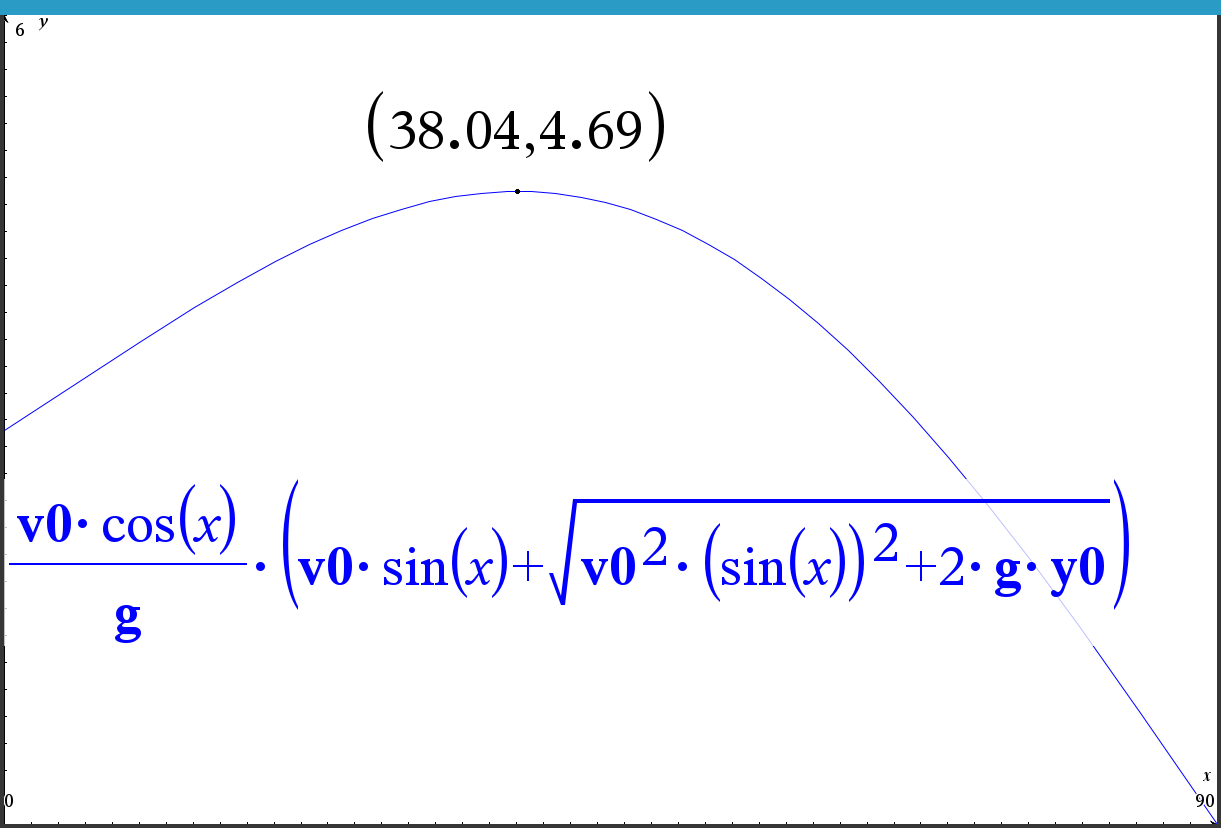
\includegraphics[width=\linewidth]{Figure 1.png}
        \end{figure}
        \begin{figure}[H]
            \caption{Numerical extremization of $R(v_0 + \sigma_{v_0}, \theta)$}
            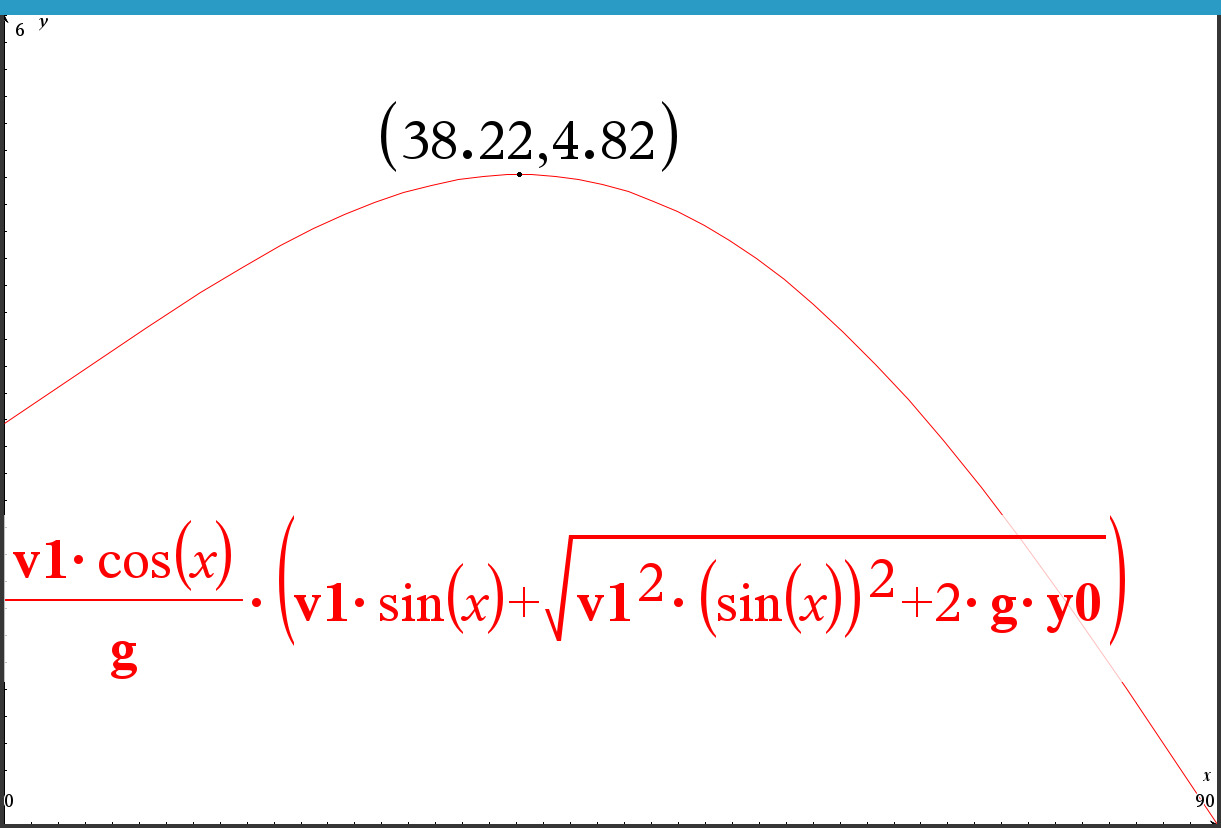
\includegraphics[width=\linewidth]{Figure 2.png}
        \end{figure}
    \section{Calculations}
    \begin{alignat*}{3}
        (1) \> &R &&= v_{0x} t \\
        &t &&= \frac{R}{v_{0x}} \\
        &y_{f} &&= y_i + v_it-\frac{1}{2}gt^2 \\
        &0 &&= y_0 + v_{0y}\left(\frac{R}{v_{0x}}\right) - \frac{1}{2}g \left(\frac{R}{v_{0x}}\right)^2\\
        &\frac{R}{v_{0x}} &&= \frac{v_{0y}+\sqrt{(v_{0y})^2-2gy_{0}}}{g}\\
        &R &&= \frac{v_{0x}}{g}\left(v_{0y}+\sqrt{(v_{0y})^2-2gy_{0}}\right)\\
        &v_{0y} &&= v_0 \sin(\theta)\\
        &v_{0x} && = v_0 \cos(\theta)\\
        &R &&= \frac{v_0 \cos(\theta)}{g}\left(v_0 \sin(\theta) +\sqrt{(v_0 \sin(\theta))^2-2gy_{0}}\right)\\\\
        \hline\\
        (2) \> &\frac{\sigma_{y0}}{y_0} && = 0.0215\%\\
        &\frac{\sigma_{R0}}{R_0} && = 1.68\%\\\\
        \hline\\
        (3) \> &\theta && = 0\\
        &|\overrightarrow{v_0}| && = v_0\cos(0)\hat{i}+v_0\sin(0)\hat{j}\\
        &&&=v_0\\
        &R_0 &&= v_0t\\
        &t = &&\frac{R_0}{v_0}\\
        &y_0 && = \frac{1}{2}gt^2\\
        &&& = \frac{1}{2}g\left(\frac{R_0}{v_0}\right)^2\\
        &v_0 && = R_0\sqrt{\frac{g}{2y_0}}\\
        &&& = 2.925 \, \text{m} \sqrt{\frac{9.8\, \mathrm{m/s^{2}} }{(2)( 1.162825\,\mathrm{m})}}\\
        &&& = 6.00 \,\mathrm{\frac{m}{s^2}}\\\\
        \hline\\
        (4)\>& v_{0R} && = 2.973 \, \text{m} \sqrt{\frac{9.8\, \mathrm{m/s^{2}} }{(2)( 1.162825\,\mathrm{m})}}\\
        &&& = 6.10 \,\mathrm{\frac{m}{s^2}}\\
        &\sigma_{v0}^2 && = (v_0R-v_0)^2\\
        &&& = \left(0.10 \, \mathrm{\frac{m}{s}}\right)^2\\
        &\sigma_{v0} && = 0.10\, \mathrm{\frac{m}{s}}\\\\
        \hline\\
        (5)\>& R_{max} &&= 4.69 \, \mathrm{m}\\
        &R^+(\theta) && = R(v_0 + \sigma_{v_0}, \theta)\\
        &&& = \frac{(v_0 + \sigma_{v_0}) \cos(\theta)}{g}\left((v_0 + \sigma_{v_0}) \sin(\theta) +\sqrt{((v_0 + \sigma_{v_0}) \sin(\theta))^2-2gy_{0}}\right)\\
        &R^+_{max} && = 4.82 \, \mathrm{m}\\
        &\sigma_{R_{max}} && = | R^+_{max} - R_{max} |\\
        &&& = 0.13 \mathrm{m}\\\\
        \hline\\
        (6)\>&\theta_{max} && = 38.04 \degree\\
        &\theta^+_{max} && = 38.22 \degree\\
        &\sigma_{\theta_{max}} && = | \theta^+_{max} - \theta_{max} |\\
        &&& = 0.18 \degree
    \end{alignat*}
    \section{Conclusion}
    No measurements had greater error than was to be expected from random error based on the precision of the meter sticks and the theoretical 
    values of the range at the angles \(\theta_{max}\), \(\theta_{max}+10\degree\), and \(\theta_{max} - 10 \degree\) are all within one or two 
    standard deviations of the experimental values for the range at those angles. Additionally random error may have arisen from 
    the slight differences in the direction of the projectile launcher as a result of the force of the decompression of the 
    spring causing the launcher to shake or from differences in the spinning of the ball in the air.
\end{document}